\documentclass[a4paper, 11pt, notitlepage]{report}

\usepackage[utf8]{inputenc}
\usepackage[T1]{fontenc}   
\usepackage[english]{babel}
\usepackage{hyperref}
\usepackage{listings}
%\usepackage{inconsolata}
\usepackage[pdftex]{graphicx}
\usepackage{color}
\usepackage[svgnames]{xcolor}
\usepackage{helvet}
\usepackage{float}
\usepackage{fullpage}

\usepackage[squaren, Gray, cdot]{SIunits}
\usepackage{array,multirow,makecell}
\setcellgapes{1pt}
\makegapedcells
\newcolumntype{R}[1]{>{\raggedleft\arraybackslash }b{#1}}
\newcolumntype{L}[1]{>{\raggedright\arraybackslash }b{#1}}
\newcolumntype{C}[1]{>{\centering\arraybackslash }b{#1}}


% You have to pass this option to texify.exe "--tex-option=-shell-escape"
% And install pygmentize: https://pypi.python.org/pypi/Pygments
\usepackage{minted}
\usemintedstyle{friendly}
\fvset{fontsize=\footnotesize} 

\setlength{\parskip}{\baselineskip}
% http://stackoverflow.com/questions/2318598/how-to-reduce-the-seperation-from-other-text-using-latex-minted
\setlength\partopsep{-\topsep}
\addtolength\partopsep{-\parskip}
\addtolength\partopsep{0.3cm}

\newminted{console}{frame=lines, tabsize=4}
\newminted{c}{frame=lines, tabsize=4, showtabs=false}
\newminted{cpp}{frame=lines, tabsize=4, showtabs=false}
\newminted{ruby}{frame=lines, tabsize=2, showtabs=false}
\newminted{irb}{frame=lines, tabsize=2, showtabs=false}
\newminted{objdump}{bgcolor=bg, frame=lines, tabsize=4}
\newminted{nasm}{frame=lines, tabsize=4}
\newminted{text}{frame=lines, tabsize=4}
\newminted{diff}{frame=lines, tabsize=4}
\newminted{python}{frame=lines, tabsize=4}
\newminted{pycon}{frame=lines, tabsize=4}
\newminted{postscript}{frame=lines, tabsize=4}

\sloppy

\hypersetup{
    unicode=true,
    pdfversion=1.7,
    pdfauthor={Emilien Girault},
    pdftitle={Solution du challenge SSTIC 2013},
    colorlinks=true,
    linkcolor=Teal,
    urlcolor=blue
}

% Alias persos
\newcommand{\footurl}[1]{\footnote{\url{#1}}}
\newcommand{\ps}[1]{\mint{postscript}|#1|}

% Import a picture:
%\begin{figure}[h!]
%  \centering
%  \includegraphics[width=0.8\textwidth]{images/wireshark-archive}
%  \caption{Extrait de l'archive chiffrée}
%  \label{wireshark-archive}
%\end{figure}

% Consol code:
%\begin{consolecode}
%\end{consolecode}

% Text code
%\begin{textcode}
%\end{textcode}

% Python code
%\begin{pyconcode}
%\end{pyconcode}

% Embed a source code
%\inputminted[frame=lines, linenos=true]{python}{code.py}

\setcounter{secnumdepth}{3}

\title{Obfuscation of steel\footnote{Ironic, of course}: meet my \textit{Kryptonite}}
\author{Axel "0vercl0k" Souchet}
\date{July 6, 2013}

\begin{document}

\maketitle
\vspace{2cm}
\begin{abstract}
For several months, I came across a lot of papers that use the LLVM framework to develop really cool tools like:
\begin{itemize}
\item decompilation framework (\href{http://llvm.org/devmtg/2013-04/bougacha-slides.pdf}{Dagger}),
\item universal deobfuscation (\href{http://opticode.coseinc.com/documents/OptiCode_Technical_Details.pdf}{Opticode}),
\item bug-finding with static binary instrumentation (\href{http://clang.llvm.org/docs/AddressSanitizer.html}{AddressSanitizer}),
\item fast C compiler (\href{http://clang.llvm.org/}{Clang}),
\item automatic test cases generator (\href{http://klee.llvm.org/}{Klee}),
\item etc.
\end{itemize}
In other words, LLVM is everywhere, and it's only the beginning.\\
In this paper, I will try in a first part, to give you an overview of the framework: basically what you can do with it and what you cannot. Then, I will introduce a PoC called \textit{Kryptonite}: a small obfuscater based on LLVM. We will talk about how you can build such tools and how they can be improved.
I'm currently playing with the version 3.3 of LLVM (the latest when I'm writing this paper), so the code may changed a bit for the upcoming version (don't hesitate to shoot me an email if this is the case).\\

Keep in mind that no CPUs were harmed during this piece of research, trust me.
\end{abstract}

\setcounter{tocdepth}{4}
\tableofcontents

\newpage
\chapter{LLVM's overview}
\section{Introduction}
The Low Level Virtual Machine project originally started years ago at the University of Illinois under the supervision of Vikram Adve and Chris Lattner (the maintainer). The purpose of the project was to build a framework to ease compiler and code generator writing. This infrastructure is written in C++ and is open-source: see the website \href{http://llvm.org/}{llvm.org}. But over the years, LLVM has really been improved by the community and Apple (mainly because they hired Chris and formed a team to work on LLVM): a lot of frontends are now available (C, C++, Objective-C, Ada, Haskell, etc.) and same thing for the backends (x86, x86\_64, ARM, MBlaze, MIPS, PPC32, PPC64, Sparc, etc.). LLVM is also:
\begin{itemize}
	\item Near from 2000 files (header and code files) ;
	\item Around 2300 classes ;
	\item Around 770 000  lines.
\end{itemize}
Yes, it is quite a huge code base and a complex piece of software, and that is exactly the reason I wanted to write something about it. You have to spend hours to read the source code, to read tutorials and to debug your buggy code ; I hope to give you enough materials to play safely with LLVM without reading tons of code :-).

As I said, the purpose of this part is to go through some fundamental concepts and tools to understand how LLVM finally works. I will also try to give you some codes, some examples because that's what matters. Keep in mind I am not an LLVM expert  at all, I may misuse this wonderful tool ; if this is the case don't hesitate to shoot me an email, I will be glad to update the paper with the good way of how things should be done!

By the way, if you don't want to compile yourself either the LLVM or the \href{http://clang.llvm.org/}{clang} code, they have kindly uploaded already-compiled binaries here: \href{http://llvm.org/releases/download.html#3.3}{Pre-built binaries}, go grab one!\\
I guess we are done for the introduction, make yourself comfortable, let's go! 

\section{The pipeline}
One of the LLVM's strengths is the modularity. It is made of essentially three very important parts: the frontend, the optimization passes, and the backend. Each of them has a very particular role in the compilation process, I will describe their roles in the following sections.

You can see each part as a black box that takes an input and produces an output, and usually that output is also the input of another black box: you can see that as a chain.
\begin{figure}[H]
  \centering
  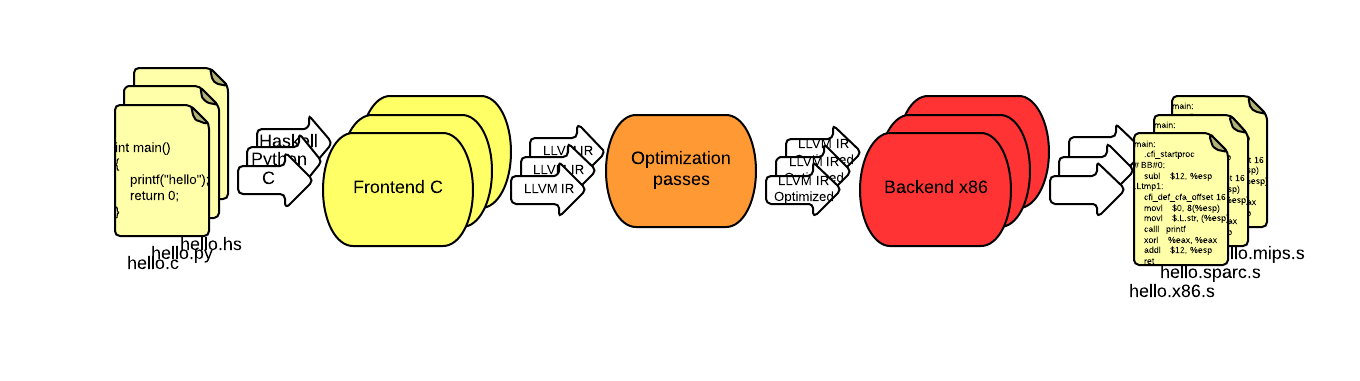
\includegraphics[width=\textwidth]{pics/pipeline.png}
  \caption{Compilation process}
\end{figure}

Note this design in three parts is not really new, the \href{http://gcc.gnu.org/}{GNU Compiler} already used this architecture.

\subsection{Frontend}
The frontend is the part you are interested in if you want to write a compiler, or if you want to tweak an existing compiler. This part takes in input a file that will be parsed by your frontend module, and your this module is responsible to generate the equivalent code using the \href{http://llvm.org/docs/LangRef.html}{LLVM Intermediate representation}. The LLVM-IR is a really important thing: basically it is a language that will be used between the output of the frontend until reaching the input of the backend. This language aims to provide several important characteristics like:
\begin{itemize}
	\item \href{http://en.wikipedia.org/wiki/Static_single_assignment_form}{SSA-form} based,
	\item type safety,
	\item low-level operations,
	\item simplicity,
	\item the capability of representing high-level languages.
\end{itemize}

To emit this LLVM-IR, you can use a dedicated API that will allow you to create instructions: if you want to see the type of instructions available the LLVM-IR read the \href{http://llvm.org/docs/LangRef.html}{LLVM Language Reference Manual}. If you want to see a real frontend, you can check \href{http://clang.llvm.org/}{Clang}'s sources: this is maybe the most famous LLVM based frontend. Its role is to rewrite the C code into the LLVM-IR using the LLVM's dedicated API I talked you about. As far as I know the frontend API is also available in \href{https://llvm.org/viewvc/llvm-project/llvm/trunk/include/llvm-c/}{C}, in \href{https://llvm.org/viewvc/llvm-project/llvm/trunk/bindings/ocaml/}{OCaml} and in \href{https://llvm.org/viewvc/llvm-project/llvm/trunk/bindings/python/}{Python} (check those slides: \href{http://fr.slideshare.net/mdevan/llvmpy-w}{llvm-py, PyCon India, 2010}) via bindings.

If you never seen the classical \textit{hello-world} in LLVM-IR, here it is:
\begin{consolecode}
@.str = private unnamed_addr constant [13 x i8] c"Hello world\0A\00", align 1

define i32 @main() {
  %1 = call i32 (i8*, ...)* @printf(i8* getelementptr inbounds ([13 x i8]* @.str, i32 0, i32 0))
  ret i32 0
}

declare i32 @printf(i8*, ...)
\end{consolecode}
You can use your preferred language to write the \textit{hello-world}, and then ask your frontend to output the LLVM-IR. To do that with \href{http://clang.llvm.org/}{clang} you just have to run it like this:
\begin{consolecode}
$ clang -S -emit--lvm hello.c -o hello.il
\end{consolecode}

Once you are able to generate this LLVM-IR you can use the rest of LLVM's pipeline without modifications: building an ELF binary for SPARC is not a problem for example (because the \href{https://llvm.org/viewvc/llvm-project/llvm/trunk/lib/Target/Sparc/}{SPARC backend} already exists).
\subsubsection[Emitting LLVM-IR via the C API]{Emitting LLVM-IR via the C API\protect\footnote{Of course you can do exactly the same with the C++ API, but in my opinion the C API is easier to understand :-).}}
Before playing with the frontend API, you have to understand a bit how the API works. First, you have to know the core of LLVM is written in C++ (you can read it in the directory \href{https://llvm.org/viewvc/llvm-project/llvm/trunk/include/llvm/}{include/llvm}) but they made also a C API built on the top of it (in the directory \href{https://llvm.org/viewvc/llvm-project/llvm/trunk/include/llvm-c/}{include/llvm-c}).

Another important detail is when you are playing with LLVM you have to manipulate several type of containers, let me describe the main ones:
\begin{enumerate}
	\item A module is a container of function and global variables, it is the equivalent of a .c file for example. This is really the top-level container used to store all the information of all other LLVM-IR objects. If you want to look at the declaration of the \textit{llvm::Module} class see \href{https://llvm.org/viewvc/llvm-project/llvm/trunk/include/llvm/IR/Module.h?view=markup}{include/llvm/IR/Module.h},
	\item A function is a container of basic-blocks: see the declaration of \textit{llvm::Function} in \href{https://llvm.org/viewvc/llvm-project/llvm/trunk/include/llvm/IR/Function.h?view=markup}{include/llvm/IR/Function.h},
	\item A basic block is a container of instructions: the declaration of \textit{llvm::BasicBlock} and \textit{llvm::Instruction} are there: \href{https://llvm.org/viewvc/llvm-project/llvm/trunk/include/llvm/IR/BasicBlock.h?view=markup}{include/llvm/IR/BasicBlock.h} and \href{https://llvm.org/viewvc/llvm-project/llvm/trunk/include/llvm/IR/Instruction.h?view=markup}{include/llvm/IR/Instruction.h}.
\end{enumerate}

As we said previously, the top-level container is the \textit{llvm::Module} class, so let's create one via \href{https://llvm.org/viewvc/llvm-project/llvm/trunk/include/llvm-c/Core.h?view=markup}{LLVMModuleCreateWithName} like that (and don't forget to clean the memory with \href{https://llvm.org/viewvc/llvm-project/llvm/trunk/include/llvm-c/Core.h?view=markup}{LLVMDisposeModule} as said in the comments) :
\begin{ccode}
LLVMModuleRef Module = LLVMModuleCreateWithName("module-c");
/// Do things with Module
LLVMDisposeModule(Module);
\end{ccode}

Once we have our module, we need to create a function via \href{https://llvm.org/viewvc/llvm-project/llvm/trunk/include/llvm-c/Core.h?view=markup}{LLVMAddFunction} ; but if you look at its declaration you see that we need first to create the type of our function. The type of a function is the number and the type of its arguments, and the type of its return value. Let's define the type of our main function with \href{https://llvm.org/viewvc/llvm-project/llvm/trunk/include/llvm-c/Core.h?view=markup}{LLVMFunctionType}, and add it to our module:
\begin{ccode}
/// void main(void)
LLVMTypeRef MainFunctionTy = LLVMFunctionType(
    LLVMVoidType(),
    NULL,
    0,
    false
);

LLVMValueRef MainFunction = LLVMAddFunction(Module, "main", MainFunctionTy);
\end{ccode}

Before going further, we still need to impor,t somehow, the \textit{printf} function:

\begin{ccode}
/// extern int printf(char*, ...)
LLVMTypeRef PrintfArgsTyList[] = { LLVMPointerType(LLVMInt8Type(), 0) };
LLVMTypeRef PrintfTy = LLVMFunctionType(
    LLVMInt32Type(),
    PrintfArgsTyList,
    0,
    true
);

LLVMValueRef PrintfFunction = LLVMAddFunction(Module, "printf", PrintfTy);
\end{ccode}

Now, we can instantiate a basic block via \href{https://llvm.org/viewvc/llvm-project/llvm/trunk/include/llvm-c/Core.h?view=markup}{LLVMAppendBasicBlock}, and create a builder via \href{https://llvm.org/viewvc/llvm-project/llvm/trunk/include/llvm-c/Core.h?view=markup}{LLVMCreateBuilder}. A builder is an object that helps you to create LLVM-IR instructions: you specify in which basic block you want to add an instruction, and you ask the builder to create one: convenient for us.
\begin{ccode}
// An instruction builder represents a point within a basic block and is
// the exclusive means of building instructions using the C interface.
LLVMBuilderRef Builder = LLVMCreateBuilder();
LLVMBasicBlockRef BasicBlock = LLVMAppendBasicBlock(MainFunction, "entrypoint");
LLVMPositionBuilderAtEnd(Builder, BasicBlock);
\end{ccode}

Perfect, we are now ready to insert real instructions. For the classic \textit{hello-world} we just need to add a global variable that will hold our string, to build a \textit{call}-like instruction, and a \texttt{ret}-like instruction (all basic blocks must be terminated by a branch instruction). Again, the C API is very simple to use:
\begin{ccode}
LLVMValueRef Format = LLVMBuildGlobalStringPtr(
    Builder,
    "Hello, %s.\n",
    "format"
), World = LLVMBuildGlobalStringPtr(
    Builder,
    "World",
    "world"
);

/// printf("Hello, %s!", world);
LLVMValueRef PrintfArgs[] = { Format, World };

LLVMBuildCall(
    Builder,
    PrintfFunction,
    PrintfArgs,
    2,
    "printf"
);

/// return;
LLVMBuildRetVoid(Builder);
\end{ccode}

Now, we need to compile our \textit{hello-world} frontend with \href{http://clang.llvm.org/}{clang++} like this:
\begin{consolecode}
$ clang++ -x c llvm-c-frontend-hello.c `llvm-config --cxxflags --ldflags --libs` -o ./llvm-c-hello
$ ./llvm-c-hello
; ModuleID = 'module-c'

@format = private unnamed_addr constant [12 x i8] c"Hello, %s.\0A\00"
@world = private unnamed_addr constant [6 x i8] c"World\00"

declare i32 @printf(...)

define void @main() {
entrypoint:
  %printf = call i32 (...)* @printf(
    i8* getelementptr inbounds ([12 x i8]* @format, i32 0, i32 0),
    i8* getelementptr inbounds ([6 x i8]* @world, i32 0, i32 0)
  )
  ret void
}
\end{consolecode}

You can even use the tool \textit{lli} (we will talk more about this tool in the backend part) to really execute the LLVM-IR code we just emitted:
\begin{consolecode}
$ ./llvm-c-hello 2>&1 | lli
Hello, World.
\end{consolecode}
OK so now you know a bit more about how a LLVM frontend looks like. If you want another example, I have made the \textit{strlen} function to see how to build if/else branches: \href{https://github.com/0vercl0k/stuffz/blob/master/llvm-funz/llvm-c-frontend-playing-with-ir.c}{llvm-c-frontend-playing-with-ir.c}. Also writing a frontend for a toy language like those ones is a cool exercise: \href{http://en.wikipedia.org/wiki/Whitespace_(programming_language)}{whitespace}, \href{http://en.wikipedia.org/wiki/Esoteric_programming_language#Piet}{piet}, \href{http://en.wikipedia.org/wiki/Shakespeare_(programming_language)}{shakespear}, etc.

\subsection{Transformation passes}
Basically, transformation passes can be of two types: either it really transforms the program (a transform pass), or either it's only reading and collecting information about your code (an analysis pass). For example, it exists a pass called "\href{https://llvm.org/viewvc/llvm-project/llvm/trunk/lib/Analysis/CFGPrinter.cpp?view=markup}{dot-cfg-only}" that generates the CFG of each function you have in your LLVM-IR file ; this is an analysis pass:
\begin{figure}[H]
  \centering
  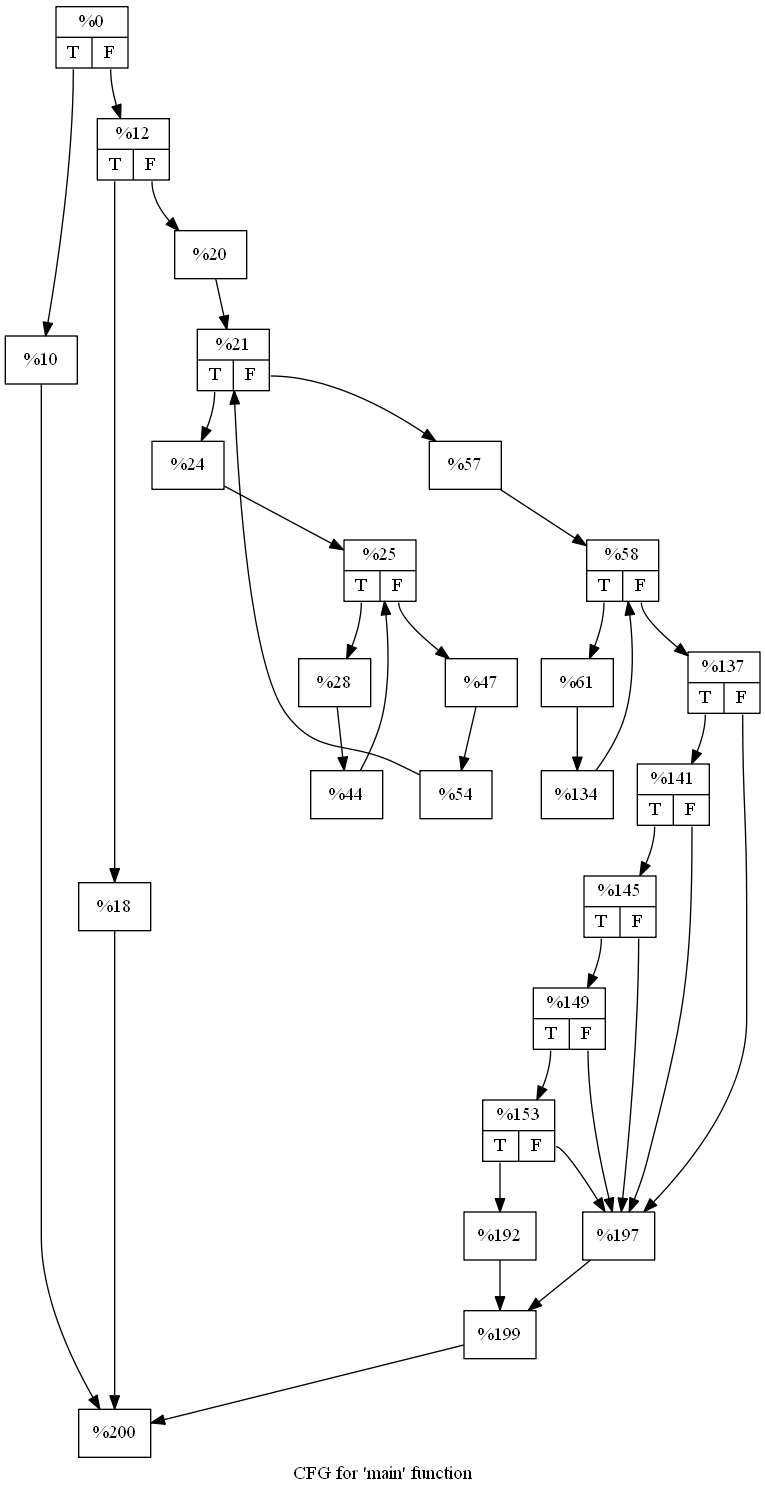
\includegraphics[scale=0.2]{pics/cfg.png}
  \caption{CFG-only of main}
\end{figure}
But at the opposite, you can also have passes that will do real optimization or transformation of your code: for example the "\href{https://llvm.org/viewvc/llvm-project/llvm/trunk/lib/Transforms/Scalar/DCE.cpp?view=markup}{Dead Code Elimination}" pass. It will go through your LLVM-IR code to find unreachable piece of code to remove them in order to simplify the program. If you want to look at the source code of the different passes, you can check the \href{https://llvm.org/viewvc/llvm-project/llvm/trunk/lib/Analysis/}{lib/Analysis} directory for analysis passes, and the \href{https://llvm.org/viewvc/llvm-project/llvm/trunk/lib/Transforms/}{lib/Transforms} for the transform passes.

When you are playing with this part of the pipeline, the important tool to know is \href{http://llvm.org/docs/CommandGuide/opt.html}{opt}: the LLVM optimizer. It is the tool that will apply the different passes you want, and will give you the optimized LLVM-IR code. Of course, it is also possible to extend its functionalities by writing new passes ; the tool is able to load dynamically your pass and to execute it to apply some analysis or transformation operations. You can enumerate all the available passes by calling this command:

\begin{consolecode}
$ opt --help
OVERVIEW: llvm .bc -> .bc modular optimizer and analysis printer
[...]
  Optimizations available:
    -aa-eval                                   - Exhaustive Alias Analysis Precision Evaluator
    -adce                                      - Aggressive Dead Code Elimination
    -alloca-hoisting                           - Hoisting alloca instructions in non-entry blocks to the entry block
[...]
\end{consolecode}
On my machine I can count exactly 157 different passes. As an example, we can try to optimize the generated LLVM-IR code for the \textit{strlen} function I gave you in the previous part (\href{https://github.com/0vercl0k/stuffz/blob/master/llvm-funz/llvm-c-frontend-playing-with-ir.c}{llvm-c-frontend-playing-with-ir.c}). Here is the code generated by our frontend:
\begin{textcode}
$ cat strlen.ll
define i32 @strlen(i8* %s) {
init:
  %i = alloca i32
  store i32 0, i32* %i
  br label %check

check:                                            ; preds = %body, %init
  %0 = load i32* %i
  %1 = getelementptr i8* %s, i32 %0
  %2 = load i8* %1
  %3 = icmp ne i8 0, %2
  br i1 %3, label %body, label %end

body:                                             ; preds = %check
  %4 = load i32* %i
  %5 = add i32 %4, 1
  store i32 %5, i32* %i
  br label %check

end:                                              ; preds = %check
  %6 = load i32* %i
  ret i32 %6
}
\end{textcode}

The function is really simple: it loops until it finds a null byte and meanwhile it increments a counter to have the len of the string. Now let's launch \href{http://llvm.org/docs/CommandGuide/opt.html}{opt} to optimize the previous code:
\begin{textcode}
$ opt -S -p -O3 strlen.ll
; ModuleID = 'strlen.ll'

; Function Attrs: nounwind readonly
define i32 @strlen(i8* nocapture %s) {
init:
  br label %check

check:                                            ; preds = %check, %init
  %storemerge = phi i32 [ 0, %init ], [ %3, %check ]
  %0 = getelementptr i8* %s, i32 %storemerge
  %1 = load i8* %0
  %2 = icmp eq i8 %1, 0
  %3 = add i32 %storemerge, 1
  br i1 %2, label %end, label %check

end:                                              ; preds = %check
  ret i32 %storemerge
}
\end{textcode}

We can clearly see the code has been quite optimized by the utility using the "\href{http://llvm.org/docs/LangRef.html#i-phi}{Phi nodes}". In this specific case you can understand the instruction as "if the execution flow comes from the basic block \textit{init}, the value zero is moved in the variable \textit{\%storemerge} ; if it comes from the basic block \textit{\%check}, the variable \textit{\%3} is moved in \textit{\%storemerge}.

In the second part of the paper, we will talk more in details about how you can write your own pass.
\subsection{Backend}
The last part of the pipeline is the backend: it is basically the software component that will traduce the LLVM-IR into the machine code for a specific CPU. We can have a list of the stable and already existing backend available in LLVM by using the tool \href{http://llvm.org/docs/CommandGuide/llc.html}{llc} (the LLVM compiler):
\begin{consolecode}
$ llc --version
LLVM (http://llvm.org/):
  LLVM version 3.3
  Optimized build.
  Default target: i386-pc-linux-gnu
  Host CPU: corei7

  Registered Targets:
    aarch64  - AArch64
    arm      - ARM
    cpp      - C++ backend
    hexagon  - Hexagon
    mblaze   - MBlaze
    mips     - Mips
    mips64   - Mips64 [experimental]
    mips64el - Mips64el [experimental]
    mipsel   - Mipsel
    msp430   - MSP430 [experimental]
    nvptx    - NVIDIA PTX 32-bit
    nvptx64  - NVIDIA PTX 64-bit
    ppc32    - PowerPC 32
    ppc64    - PowerPC 64
    sparc    - Sparc
    sparcv9  - Sparc V9
    systemz  - SystemZ
    thumb    - Thumb
    x86      - 32-bit X86: Pentium-Pro and above
    x86-64   - 64-bit X86: EM64T and AMD64
    xcore    - XCore
\end{consolecode}
This tool is very handy: you give it an LLVM-IR module for example and it is capable of generating the assembly according to the target you have chosen. As an example, we can try to compile our \textit{hello-world} LLVM-IR program into \href{http://en.wikipedia.org/wiki/X86}{x86} and \href{http://en.wikipedia.org/wiki/MIPS_architecture}{MIPS}:
\begin{consolecode}
$ llc hello.ll -march=mips -o hello.mips.s
$ llc hello.ll -march=x86 -o hello.x86.s
$ cat hello.x86.s
# [...]
main:                                   # @main
        .cfi_startproc
# BB#0:                                 # %entrypoint
        subl    $12, %esp
.Ltmp1:
        .cfi_def_cfa_offset 16
        movl    $.Lworld, 4(%esp)
        movl    $.Lformat, (%esp)
        calll   printf
        addl    $12, %esp
        ret
# [...]
$ cat hello.mips.s
main:
# [...]
# BB#0:                                 # %entrypoint
        lui     $2, %hi(_gp_disp)
        addiu   $2, $2, %lo(_gp_disp)
        addiu   $sp, $sp, -24
$tmp2:
        .cfi_def_cfa_offset 24
        sw      $ra, 20($sp)            # 4-byte Folded Spill
$tmp3:
        .cfi_offset 31, -4
        addu    $gp, $2, $25
        lw      $1, %got($format)($gp)
        addiu   $4, $1, %lo($format)
        lw      $1, %got($world)($gp)
        lw      $25, %call16(printf)($gp)
        jalr    $25
        addiu   $5, $1, %lo($world)
        lw      $ra, 20($sp)            # 4-byte Folded Reload
        jr      $ra
        addiu   $sp, $sp, 24
# [...]
\end{consolecode}
Of course, once you got those assembly files you can just use whatever compiler you like to generate an executable binary. Here is an example with \href{http://clang.llvm.org/}{clang}:
\begin{consolecode}
$ clang hello.x86.s -o hello
$ file hello
hello: ELF 32-bit LSB executable, Intel 80386, version 1 (SYSV), dynamically linked (uses shared libs),
for GNU/Linux 2.6.26, not stripped
$ ./hello
Hello, World.
\end{consolecode}
If you have to create your own CPU target, this is surely the hardest part: it exists some really good tutorials but creating its own backend (even for a toy-cpu) is clearly tough.

Another other interesting part, is the JIT compiler engine that you can use directly via the \href{http://llvm.org/docs/CommandGuide/lli.html}{lli} tool. This tool allows you to take an LLVM-IR file, to JIT compile the code and to directly execute it. Basically, if you are on an x86 host computer, the \href{http://llvm.org/docs/CommandGuide/lli.html}{lli} program will JIT compile the code using the x86 backend and will run it. We can try to execute our \textit{hello-world} program:
\begin{consolecode}
$ lli hello.ll
Hello, World.
\end{consolecode}

\subsection{Conclusion and going further}
As you can see previously, LLVM is a really cool set of libraries to implement compiler or JIT compiler. What's really nice is to be able to only implement only the part you need and once it is done you can use what already exists: frontends, optimization passes or backends. Though some parts may be a bit obscure and not really trivial to play with, that's why I did a little list of interesting links you should read if you definitely want to go further (yeah, it was only a small introduction):
\begin{itemize}
	\item \href{http://llvm.org/docs/tutorial/LangImpl1.html}{Kaleidoscope: Implementing a Language with LLVM}: if you want to write a frontend, read this, it's perfect
	\item \href{http://llvm.org/docs/WritingAnLLVMPass.html}{Writing an LLVM Pass}: it gives you the basics to write your own analysis/transform pass
	\item \href{http://jonathan2251.github.io/lbd/}{Creating an LLVM Backend for the Cpu0 Architecture}: this one focus the backend part ; it's very tough but it is a really good tutorial
\end{itemize}

\newpage
\chapter{Kryptonite}
\section{Introduction}
The first time I saw the LLVM's pipeline picture, I was really interested in the LLVM-IR and by the passes parts. It is clearly here you want to play if you are interested in obfuscation, because you deal with the LLVM-IR and not the target CPU assembly. Basically it means your obfuscation can be reused by all the backends supported by LLVM. You can simply write your code in C, then you ask clang to generate the LLVM-IR code and from there you can really transform the LLVM-IR the way it pleases you. Once you are done: you just have to compile it for the CPU you target. Usually, when we see obfuscaters either the authors are modifying the source (and it is usable only for one language), or either it does the obfuscation at the assembly level: in this case it is CPU specific (you have also lot of problems with the instruction side-effects). In our case, you can use the language you want, among the available LLVM frontends of course, and your obfuscation ideas can be reused for others targets. You will see in that part we will not need to hack clang's sources, or to mess with the code's AST to generate heavy obfuscated binaries.

The purpose of this part is just to show you the small PoC I have written for the fun. You will, of course, find the sources of the project on my \href{https://github.com/0vercl0k/stuffz/tree/master/llvm-funz/kryptonite}{github} account. By the way, I have prepared a little crackme that has been obfuscated with my tool \textit{Kryptonite} to illustrate what type of binaries it can produce. 
\section{Writing an optimization pass}
Before talking about the obfuscation part, we need to know how you are supposed to build an optimization pass. In a nutshell, it is a simple shared dynamic libraries that will be loaded by \href{http://llvm.org/docs/CommandGuide/opt.html}{opt}, the LLVM optimizer. If you read carefully, the \href{http://llvm.org/docs/WritingAnLLVMPass.html}{Writing an LLVM Pass} tutorial on the LLVM's wiki, you see that a pass can be involved at several levels. By levels, I mean that you can create a pass to optimize basic blocks, to transform functions, or to optimize a whole module. To do so, you have to subclass the according LLVM class and to implement some specific routines: \href{https://llvm.org/viewvc/llvm-project/llvm/trunk/include/llvm/Pass.h?view=markup}{llvm::FunctionPass} for example. Note that you are not supposed to mess too much with the original code: for example if you choose to do a \href{https://llvm.org/viewvc/llvm-project/llvm/trunk/include/llvm/Pass.h?view=markup}{llvm::BasicBlockPass}, modifying the CFG is not authorized. So check really the documentation to be sure you don't try to do something you mustn't.

Let's try to make a \textit{hello-world} pass that will display the name of each function. As I said, earlier we need to subclass \href{https://llvm.org/viewvc/llvm-project/llvm/trunk/include/llvm/Pass.h?view=markup}{llvm::FunctionPass} and to implement the pure virtual \href{https://llvm.org/viewvc/llvm-project/llvm/trunk/include/llvm/Pass.h?view=markup}{llvm::FunctionPass::runOnFunction} method.

\begin{cppcode}
struct Hello : public llvm::FunctionPass
{
    static char ID;
    Hello()
    : FunctionPass(ID)
    {}

    bool runOnFunction(llvm::Function &F)
    {
        printf("Function being handled: %s\n", F.getName().data());
        return false;
    }
};

char Hello::ID = 0;
static llvm::RegisterPass<Hello> X("hello", "hello pass!", false, false);
\end{cppcode}

Then you can compile it, and run it through the LLVM optimizer via those commands:
\begin{consolecode}
$ clang++ hello.cpp `llvm-config --cxxflags --ldflags --libs core` -shared -o hello.so
$ opt -load ./hello.so -help | grep hello
    -hello                                     - hello pass!
\end{consolecode}

OK, now you know how to build a really basic pass. The other part is to play with the different containers I presented a bit earlier: you add instructions, you split basic blocks, you remove instructions, you insert new basic blocks ; it's simple, you just have to find the right API. Don't hesitate to check my sources, I have examples of how you can change the CFG of a function, how to insert/split basic blocks etc.

\section{LLVM-IR obfuscation}
The purpose of this section is to focus on the obfuscation, to discuss what I have implemented, and to see how we could improve the PoC.
\subsection{Obfuscate \textit{add} instructions}
My idea was quite simple, I wanted to recode the equivalent of an \textit{add} instruction but without addition. The \textit{add} instruction is really important because it is used in most of all programs, and if you think about it you can even transform some instructions to use \textit{add} instructions instead ; we will see those cases a bit later. 
\subsubsection{Theory: home made 32 bits adder}
I am pretty sure, almost all of you have already studied this younger: how to make a full 32 bits adder with only logic operators. But to do that, we have first to implement a full 1 bit adder. As you can see in the picture \ref{bit-adder}, a 1 bit adder system has 3 inputs:
\begin{itemize}
	\item $A$: the first bit you want to add
	\item $B$: the second bit you want to add
	\item $C_{in}$: the input carry (useful when chaining several 1 bit adders)
\end{itemize}
\begin{figure}[H]
  \centering
  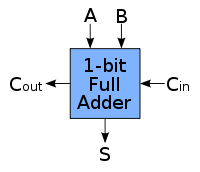
\includegraphics[scale=0.7]{pics/full-adder-1bit.png}
  \caption{Full 1 bit adder (source: wikipedia.org)}
  \label{bit-adder}
\end{figure}
And it has 2 outputs:
\begin{itemize}
	\item $S$: the solution of the addition ($A+B+C_{in}$)
	\item $C_{out}$: the output carry (this one will be introduced in the input carry of another adder)
\end{itemize}
Writing the truth table of this system gives the following:\\\\
\begin{center}
\begin{tabular}{|C{1cm}|C{1cm}|C{1cm}||C{1cm}|C{1cm}|}
  \hline
  A & B & Cin & Cout & S \\
  \hline
  0 & 0 & 0 & 0 & 0 \\
  0 & 0 & 1 & 0 & 1 \\
  0 & 1 & 0 & 0 & 1 \\
  0 & 1 & 1 & 1 & 0 \\
  1 & 0 & 0 & 0 & 1 \\
  1 & 0 & 1 & 1 & 0 \\
  1 & 1 & 0 & 1 & 0 \\
  1 & 1 & 1 & 1 & 1 \\
  \hline
\end{tabular}
\end{center}

Now if you extract both the equations of \textit{S} and \textit{Cout}, you get those ones: 
\begin{itemize}
	\item $S = \overline{A} B \overline{C_{in}} \vee A \overline{B C_{in}} \vee  \overline{A B} C_{in} \vee A B C_{in}$
	\item  $C_{out} = \overline{A} B  C_{in} \vee A \overline{B} C_{in} \vee A B \overline{C_{in}} \vee A B C_{in}$
\end{itemize}
The watchful readers will see that the second equation is not simplified, and you can ask yourself why ? That's simple, we want to produce the most awful code possible, so we really don't want to simplify it. Now we have those equations, we are able easily to write a system capable of adding two bits, that's cool.

The plan now is to make a chain of 1 bit adder in order to have a real 32 bits adder like in the picture \ref{4bitsadder} (but with 32 blocks instead of 4).
\begin{figure}[H]
  \centering
  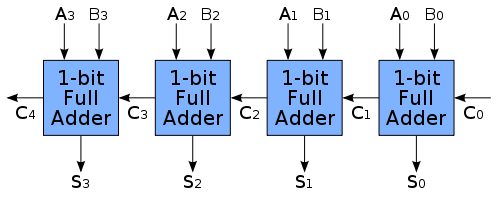
\includegraphics[scale=0.7]{pics/ripple-carry.png}
  \caption{Full 4 bits adder (source: wikipedia.org)}
  \label{4bitsadder}
\end{figure}

So this was the theory part, because we have to implement the 32 bits adder using the frontend API of LLVM to emit it in LLVM-IR as we did for the \textit{hello-world} example in the first part.

\subsubsection{Practice: Emit the adder with the LLVM frontend API}
Let's describe how to write a 1 bit adder in LLVM-IR. We need the two outputs described earlier, but we will focus on the $S$ one ($C_{out}$ is pretty much the same). Don't forget a little thing though: you have to extract the bit you want in the original two operands of the \textit{add} instructions. So if you have i32 operands A and B, the first 1 bit adder will focus on the bit n\degree 0 of both A and B ; and to do that we will have to do some bit manipulations (with right-shifts and \textit{and} masks).  Besides this detail, the LLVM-IR has all the binary operators we need, and we just have to follow the equations. We start by creating the $A$, $B$, $\overline{A}$ and $\overline{B}$ (we don't need the $C_{in}$ because we add the two LSB):

\begin{cppcode}
// LO_RShifted0 = A >> 0
llvm::Instruction *LO_RShifted0 = llvm::BinaryOperator::CreateLShr(
    A, llvm::ConstantInt::get(Int32Ty, 0),
    "", bbl
);
// LO_RShiftedAnded0 = (A >> 0) & 1 = bit0 of A
llvm::Instruction *LO_RShiftedAnded0 = llvm::BinaryOperator::CreateAnd(
    LO_RShifted0, llvm::ConstantInt::get(Int32Ty, 1),
    "", bbl
);
// LO_RShiftedAndedNoted0 = ~((A >> 0) & 1) = ~(bit0 of A)
llvm::Instruction *LO_RShiftedAndedNoted0 = llvm::BinaryOperator::CreateXor(
    LO_RShiftedAnded0, llvm::ConstantInt::get(Int32Ty, 1),
    "", bbl
);

// Same thing for B
llvm::Instruction *RO_RShifted0 = llvm::BinaryOperator::CreateLShr(
    B, llvm::ConstantInt::get(Int32Ty, 0),
    "", bbl
);
llvm::Instruction *RO_RShiftedAnded0 = llvm::BinaryOperator::CreateAnd(
    RO_RShifted0, llvm::ConstantInt::get(Int32Ty, 1),
    "", bbl
);
llvm::Instruction *RO_RShiftedAndedNoted0 = llvm::BinaryOperator::CreateXor(
    RO_RShiftedAnded0, llvm::ConstantInt::get(Int32Ty, 1),
    "", bbl
);
\end{cppcode}

Once we have our input variables ready, we can follow the equation of $S$ we saw earlier:

\begin{cppcode}
// Now we follow the equation and we build the successive AND
llvm::Instruction *R_And010 = llvm::BinaryOperator::CreateAnd(LO_RShiftedAndedNoted0, RO_RShiftedAnded0, "", bbl);
llvm::Instruction *R_And020 = llvm::BinaryOperator::CreateAnd(R_And010, llvm::ConstantInt::get(Int32Ty, 1), "", bbl);
llvm::Instruction *R_And110 = llvm::BinaryOperator::CreateAnd(LO_RShiftedAnded0, RO_RShiftedAndedNoted0, "", bbl);
llvm::Instruction *R_And120 = llvm::BinaryOperator::CreateAnd(R_And110, llvm::ConstantInt::get(Int32Ty, 1), "", bbl);
llvm::Instruction *R_And210 = llvm::BinaryOperator::CreateAnd(LO_RShiftedAndedNoted0, RO_RShiftedAndedNoted0, "", bbl);
llvm::Instruction *R_And220 = llvm::BinaryOperator::CreateAnd(R_And210, llvm::ConstantInt::get(Int32Ty, 0), "", bbl);
llvm::Instruction *R_And310 = llvm::BinaryOperator::CreateAnd(LO_RShiftedAnded0, RO_RShiftedAnded0, "", bbl);
llvm::Instruction *R_And320 = llvm::BinaryOperator::CreateAnd(R_And310, llvm::ConstantInt::get(Int32Ty, 0), "", bbl);

// ORing them
llvm::Instruction *R_Or00 = llvm::BinaryOperator::CreateOr(R_And020, R_And120, "", bbl);
llvm::Instruction *R_Or10 = llvm::BinaryOperator::CreateOr(R_And220, R_And320, "", bbl);

// Gotcha, we have the result in R0
llvm::Instruction *R0 = llvm::BinaryOperator::CreateOr(R_Or00, R_Or10, "", bbl);
\end{cppcode}
In the previous example, the variable \textit{R0} will hold the result of the addition between the bit  n\degree0 of both A and B. Now you repeat those operations 32 times to have a complete adder!

I have written a Python script that generates the 32 bits adder, you can find the script here: \href{https://github.com/0vercl0k/stuffz/blob/master/llvm-funz/generate_homemade_32bits_adder_llvm_ir.py}{generate\_homemade\_32bits\_adder\_llvm\_ir.py}. I also made a little program to emit the LLVM-IR code able to do the addition, to see how painful and how big the final assembly code is: \href{https://github.com/0vercl0k/stuffz/blob/master/llvm-funz/llvm-cpp-frontend-home-made-32bits-adder.cpp}{llvm-cpp-frontend-home-made-32bits-adder.cpp}. You can try it out yourself with those commands:
\begin{consolecode}
$ wget 'https://raw.github.com/0vercl0k/stuffz/master/llvm-funz/llvm-cpp-frontend-home-made-32bits-adder.cpp'
$ clang++ llvm-cpp-frontend-home-made-32bits-adder.cpp `llvm-config --cxxflags --ldflags --libs core` -o emit_adder
$ ./emit_adder 2> adder.ll # Now we can emit the LLVM-IR for the home made 32 bits adder
$ wc -l adder.ll
1016 adder.ll # That's only for one add instruction..:))
$ llc -O0 adder.ll -o adder.s # We can also generate the x86 assembly
$ wc -l adder.s
1956 adder.s # Instead of one add instruction :P
$ clang adder.s -o adder
$ ./adder 137 1000 # And we can run it
Result: 1137
$ ./adder 4294967295 1338
Result: 1337
\end{consolecode}

We are now able to implement a home made 32 bits adder, and I hope you saw that it generates a ton of x86 assembly line ; perfect for us. But now we want to modify the content of all basic blocks with our LLVM pass:
\begin{enumerate}
	\item match all the \textit{add} instructions in all the basic blocks of each function. To do so, you can iterate through each basic block, then through each instruction. Finally you have just to match what type of instruction it is.
	\item replace them all with our adder. You insert your different instructions just before the \textit{add} instruction you want to replace. Then, the important thing is to replace the old \textit{add} instruction with the new using the function \href{https://llvm.org/viewvc/llvm-project/llvm/trunk/include/llvm/Transforms/Utils/BasicBlockUtils.h?view=markup}{llvm::ReplaceInstWithInst}.
\end{enumerate}

Another dumb thing I have implemented is to decompose one \textit{add} instruction into hundred others as you can see on figure \ref{adds}. I did that to introduce more \textit{add} in the program, this way if I run a second time my obfuscation pass I would be able to obfuscate heavily those ones with the home made 32 bits adder.

\begin{figure}[H]
  \centering
  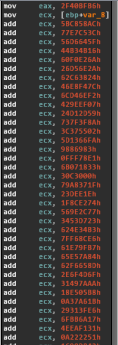
\includegraphics[scale=0.7]{pics/adds.png}
  \caption{Tons of add that could be heavily-obfuscated with a home made adder.}
  \label{adds}
\end{figure}

\subsection{Mess with other instructions}
The idea here is the same: you want to write an instruction in a different way but you want to keep the same result ; because you don't want to crash your program. Easy targets are the binary operators like \textit{mul}, \textit{sub}, \textit{xor}, etc. For example, you can recode the \textit{xor} instruction only with \textit{not}, \textit{or} and \textit{and} instructions. You can also unroll a \textit{mul} instruction into several \textit{add} instructions. This is the part where you have to be creative, and where you have to express all the anger you have for the world. This is also the not-so-fun part: that's why you will find in my PoC only two or three instructions obfuscated (it's enough for the demo crackme :-)).

Note that you can also use \href{http://rise4fun.com/z3py}{Z3py} to be sure your transformations are equivalent, or not.
\begin{consolecode}
In [1]: from z3 import *
In [2]: a = BitVec('a', 32)
In [3]: b = BitVec('b', 32)
In [4]: prove(a^b == (a&(~b)|(~a)&b))
proved
\end{consolecode}

\subsection{Inserting x86 assembly}
Another interesting thing was to be able to add directly assembly code for a specific CPU target. There is a dedicated class in the LLVM code base to do exactly that: \href{https://llvm.org/viewvc/llvm-project/llvm/trunk/include/llvm/IR/InlineAsm.h?view=markup}{llvm::InlineAsm}. Then you just have to build a \textit{call} instruction to trigger the execution of your assembly code.
\begin{textcode}
define void @main() {
  call void asm sideeffect "int3", "~{dirflag},~{fpsr},~{flags}"() #1, !srcloc !0
  ret void
}
\end{textcode}
To add a bit of fun in the demo-crackme, I decided to implement a simple ptrace-based anti-debug. I'm not really a linux guy, but I already spent some days to debug stuff in \href{http://www.gnu.org/software/gdb/}{GDB} and it's really not fun when you have \href{http://linux.die.net/man/2/fork}{fork} and \href{http://linux.die.net/man/2/ptrace}{ptrace} stuff everywhere ; so I wanted to do something with those two. In the gnu debugger, you can either follow the child process, or the parent process (the default option) via the \textit{follow-fork-mode} option. Here was my simple idea:
\begin{enumerate}
	\item The process will fork to create another process
	\item The son process will try to attach itself to the parent process using \href{http://linux.die.net/man/2/ptrace}{ptrace}
	\begin{enumerate}
		\item If it works, that's OK ; we will continue the flow of execution in the son (because the user will step in the parent, and we are nasty)
		\item If it doesn't work, we end the game: we kill both the parent and ourself
	\end{enumerate}
	\item The father will wait. He will be killed anyway by the son, to let the son execute itself
\end{enumerate}
That worked quite great in my head, but when I did try to test that on my GDB it just didn't work. After some hours of debugging, I finally noticed my .gdbinit file were telling to the debugger to follow the child process instead of the parent. That means when I will try to \href{http://linux.die.net/man/2/ptrace}{ptrace} the parent, GDB won't be attached to the parent anymore but it will be attached to the son ; that's why it didn't work in GDB but did work with \href{http://linux.die.net/man/1/strace}{strace}.
\begin{ccode}
void main()
{
    unsigned int pid, ppid;
    printf("Anti follow-fork-parent!\n");

    pid = fork();
    if(pid == 0)
    {
        printf("[Son] Hi!\n");
        ppid = getppid();
        if(ptrace(PTRACE_ATTACH, ppid, 0, 0) < 0)
        {
            printf("[Son] Father is debugged, let's kill him!");
            kill(ppid, SIGKILL);
            exit(1);
        }
        else
        {
            waitpid(ppid, NULL, 0);
            printf("[Son] Continue the son, detaching from the father & killing him\n");
            ptrace(PTRACE_DETACH, ppid, 0, 0);
            kill(ppid, SIGKILL);
        }
    }
    else
    {
        printf("[Father] Hi!, waiting my son attach\n");
        waitpid(pid, NULL, 0);
    }
    printf("Continuing now..\n");
   /* do stuff */
    printf("Done!\n");
}
\end{ccode}
So I added to my test file the exact same steps, but the way around: the father will try to attach itself on the son to detect the follow-child mode of gdb. Finally, I ended up concatenating the two in order to detect both follow-child and follow-parent behavior. Here is the second part:
\begin{ccode}
void main()
{
    unsigned int pid;
    printf("Anti follow-fork-child\n");
    pid = fork();
    if(pid == 0)
    {
        printf("[Son] Hi, waiting my father..\n");
        waitpid(getppid(), NULL, 0);
    }
    else
    {
        if(ptrace(PTRACE_ATTACH, pid, 0, 0) < 0)
        {
            printf("[Father] Son is debugged, kill him & kill myself!");
            kill(pid, SIGKILL);
            exit(0);
        }
        else
        {
            waitpid(pid, NULL, 0);
            printf("[Father] Continue the father, detaching from the son & killing him\n");
            ptrace(PTRACE_DETACH, pid, 0, 0);
            kill(pid, SIGKILL);
        }
    }

    printf("Continuing now..\n");
   /* do stuff */
    printf("Done!\n");
}
\end{ccode}

To sum up, it means you can also mess with the assembly and write really specific things for specific targets. Just make sure about the side effects of your assembly instructions, because again you don't want to break your program. Of course my previous examples are a bit dumb, you can just nop the whole things very easily, but whatever.
\subsection{Showcase: Kryptonite crackme}
Yes, what was the best thing to do to test this little obfuscater ? Try it out on a little challenge for sure!

The original one is coded is  ~60 lines of plain C and it is not using system specific stuff.
The purpose is simple: find the password that gives the 'Good boy' message ; this is not a \textit{patchme} challenge.
 You will find:
\begin{itemize}
	\item A Linux x86 binary with the little anti-debugs explained earlier (tested on a Debian 6.0 x86)
	\item A Linux x64 binary without anti-debugs (tested on a Debian 6.0 x64)
	\item A Windows x64 binary without anti-debugs (tested on a Windows 7 x64)
\end{itemize}
As an example, the linux binary has been generated with the following commands:
\begin{consolecode}
$ cp kryptonite-crackme.original.ll kryptonite-crackme.ll

$ opt -S -load ./llvm-functionpass-kryptonite-obfuscater.so -kryptonite kryptonite-crackme.ll -o \ 
kryptonite-crackme.opti.ll
$ mv kryptonite-crackme.opti.ll kryptonite-crackme.ll

$ opt -S -load ./llvm-functionpass-kryptonite-obfuscater.so -kryptonite -heavy-add-obfu -enable-anti-dbg 66 \ 
kryptonite-crackme.ll -o kryptonite-crackme.opti.ll
$ mv kryptonite-crackme.opti.ll kryptonite-crackme.ll

$ llc -O0 -filetype=obj -march=x86 kryptonite-crackme.ll -o kryptonite-crackme.o
$ clang -static kryptonite-crackme.o -o kryptonite-crackme
$ strip --strip-all ./kryptonite-crackme

$ ls -la ./kryptonite-crackme
-rwxr-xr-x 1 overclok overclok 18M 22 juil. 23:19 ./kryptonite-crackme
\end{consolecode}
All binaries are quite \textbf{fat} and \textbf{awful} to look at. Remember that was the purpose of our obfuscater :-P.\\ After one or two weeks, I will publish the original source of the crackme on my github account. If someone breaks it, I will be happy to offer him/her a beer somewhere in sometime!
\newpage
\section{Final words}
Anyway, I hope I really gave you nasty ideas, and you want now to play with LLVM. It is a really powerful/cool tool, so feel free to hack it ; but don't forget to publish your sources :-).
There are also a ton of ideas I wanted to try, if you have the courage to implement them go ahead:
\begin{itemize}
	\item play with the floating arithmetic, hopefully the compiler will generate ugly SSE instructions ; maybe we can even reuse what some of the work \href{https://twitter.com/skier_t}{skier\_t} already \href{https://github.com/jbremer/ssexy}{did}
	\item obfuscate even the standard functions and not only our functions
	\item try to generate a kernel module, or a Windows driver executable ; would be awesome
	\item doing some complicated things like CFG flattening, hide the end of the loops, code encryption, etc
	\item obfuscate C++ code, I guess it will be even scarier and bigger
	\item string encryption
	\item re-implement manually other instructions the same way we did with the \textit{add} instruction
	\item add integrity checks several watch-dog threads, to prevent the user to patch/debug the binary
	\item etc.
\end{itemize}
This is the end now guys, I hope you enjoy the read, and if you have any remarks, advises: shoot me an email or DM me on twitter.

By the way, all the binaries have been uploaded \href{http://download.tuxfamily.org/overclokblog/Obfuscation%20of%20steel%3a%20meet%20my%20Kryptonite/binaries/}{here}, and the source of \textit{kryptonite} is \href{https://github.com/0vercl0k/stuffz/blob/master/llvm-funz/kryptonite/llvm-functionpass-kryptonite-obfuscater.cpp}{here} ; have fun! I would be really happy to see solutions to defeat that massive-heavy obfuscations!

Special thanks to those guys: \href{https://twitter.com/elvanderb}{@elvanderb}, \href{https://twitter.com/gentilkiwi}{@gentilkiwi}, \href{https://twitter.com/__x86}{@\_\_x86} and \href{https://twitter.com/agixid}{@agixid}.

\begin{figure}[H]
  \centering
  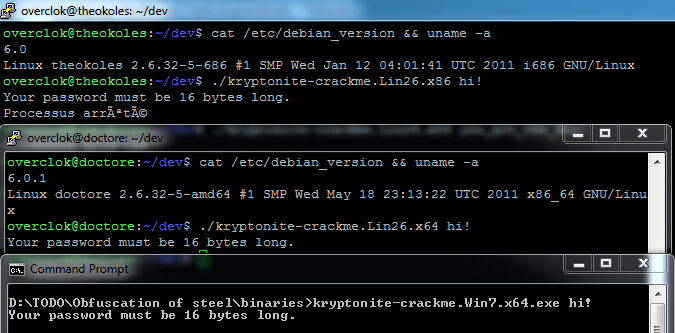
\includegraphics[scale=0.7]{pics/crackme.png}
\end{figure}
\end{document}

